% Created 2018-03-13 Die 16:35
\documentclass[ngerman,a4paper,11pt]{scrreprt}
\usepackage[utf8]{inputenc}
\usepackage[T1]{fontenc}
\usepackage{fixltx2e}
\usepackage{graphicx}
\usepackage{longtable}
\usepackage{float}
\usepackage{wrapfig}
\usepackage{rotating}
\usepackage[normalem]{ulem}
\usepackage{amsmath}
\usepackage{textcomp}
\usepackage{marvosym}
\usepackage{wasysym}
\usepackage{amssymb}
\tolerance=1000
\usepackage{natbib}
\usepackage[linktocpage,pdfstartview=FitH,colorlinks,linkcolor=blue,
anchorcolor=blue,citecolor=blue,filecolor=blue,menucolor=blue,urlcolor=blue]{hyperref}
\usepackage{ngerman}
\usepackage{graphicx}
\addtokomafont{disposition}{\rmfamily}
\newcommand{\sectionbreak}{\clearpage}
\setcounter{secnumdepth}{4}
\date{\today}
\title{}
\hypersetup{
  pdfkeywords={},
  pdfsubject={},
  pdfcreator={Emacs 25.3.1 (Org mode 8.2.10)}}
\begin{document}

\begin{titlepage}
  \setlength{\fboxsep}{50pt}
  \setlength{\fboxrule}{3pt}

  \vfill
  \vfill

  \begin{minipage}{\textwidth}
    \begin{center}
      \vspace*{4cm}
      \framebox[\textwidth][c]{
        \begin{minipage}{\textwidth}
          \begin{center}
            \vspace*{2cm}
            \huge{\textbf{\uppercase{Todesanzeigen}}}\\
            \vspace*{.3cm}
            \large{\uppercase{\textit{und}}}\\
            \vspace*{.1cm}
            \huge{\textbf{\uppercase{Danksagungen}}}\\
            \vspace*{2cm}
          \end{center}
      \end{minipage}}
    \end{center}
  \end{minipage}

  \vfill

  \begin{minipage}{\textwidth}
    \begin{center}
      \Large{\textit{Melanie Bühler}}\\
      \Large{\textit{März 2018}}\\
    \end{center}
  \end{minipage}

  \vfill

  \begin{minipage}{\textwidth}
      \centering{az-medien-Logo, ot-Logo, Stadtanzeiger Logo}
  \end{minipage}

\end{titlepage}
\newpage

\tableofcontents

\part{Todesanzeige}
\label{sec-1}

\chapter{Inhalt der Todesanzeige}
\label{sec-1-1}

\begin{itemize}
\item Name (gegebenenfalls Geburtsname) des Verstorbenen
\item Geburts- und Todesdatum
\item Ort des Todes
\item Verfasser der Anzeige
\item Informationen zur Bestattung

Wenn es in Ordnung ist, dass eine unbekannte Zahl von Trauergästen zur
Bestattung kommt, so kann man die Informationen über Termin und Ort der
Bestattung in der Todesanzeige publizieren. So erspart man es sich,
gesonderte Einladungen zu versenden.

\item Information zur Todesart

In vielen Todesanzeigen wird kurz auf den Grund für den Todesfall
eingegangen, zum Beispiel nach langer Krankheit oder durch einen tragischen
Unfall. Diese Information in der Traueranzeige kann es den Hinterbliebenen
ersparen, auf Nachfragen reagieren zu müssen, die nähere Informationen
einfordern.

\item Wünsche für die Abdankungsfeier

In der Todesanzeige kann man auch auf besondere Wünsche für die Feier
hinweisen, so zum Beispiel den Verzicht auf Blumen- oder Kranzspenden oder
die Bitte, am Grab von Beileidsbekundungen abzusehen. Wer möchte, kann eine
Organisation angeben, an die das für den Kranz gedachte Geld gespendet
werden kann. Die meisten Trauergäste werden diesen Wünschen gerne
nachkommen.
\end{itemize}

\chapter{Gliederung der Todesanzeige}
\label{sec-1-2}

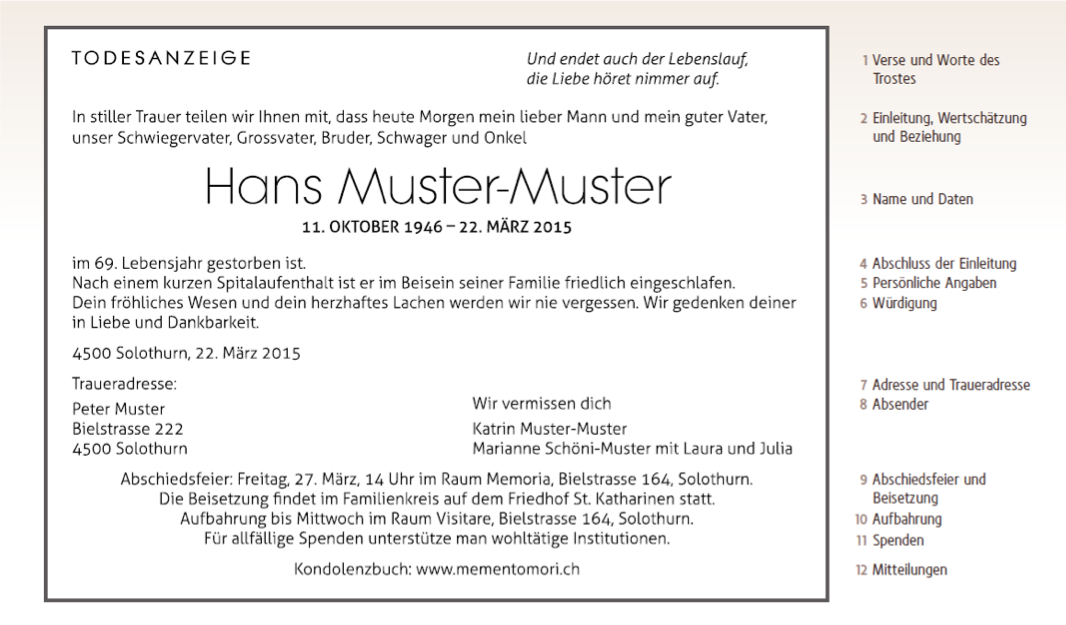
\includegraphics[width=\textwidth]{Bilder/MusterTodesanzeige.png}

\clearpage

\section{Verse und Worte des Trostes}
\label{sec-1-2-1}

\subsection{Traditionelle Trauersprüche}
\label{sec-1-2-1-1}

\begin{verse}
Auch wenn wir dir die Ruhe gönnen, \\
ist voller Trauer unser Herz. \\
Dich leiden sehen, ohne helfen zu können, \\
war für uns der grösste Schmerz. \\
\end{verse}

\begin{verse}
Die Zeit heilt nicht alle Wunden, \\
sie lehrt uns nur mit dem Unbegreiflichen zu leben. \\
\end{verse}

\begin{verse}
Du hast gesorgt, du hast geschafft, \\
bis dir die Krankheit nahm die Kraft. \\
Schlicht und einfach war dein Leben, \\
treu und fleissig deine Hand, \\
immer helfend für die Deinen, \\
ruhe sanft und habe Dank. \\
\end{verse}

\begin{verse}
Eine Stimme, die uns vertraut war, schweigt. \\
Ein Mensch, der immer für uns da war, lebt nicht mehr. \\
Erinnerung ist das, was bleibt. \\
\end{verse}

\begin{verse}
Erinnerungen sind kleine Sterne, \\
die tröstend in das Dunkel unserer Trauer leuchten. \\
\end{verse}

\begin{verse}
Es gibt im Leben für alles eine Zeit, \\
eine Zeit der Freude, der Stille, der Trauer \\
und eine Zeit der dankbaren Erinnerung. \\
\end{verse}

\begin{verse}
Ganz still und leise, ohne ein Wort, \\
gingst du von deinen Lieben fort, \\
du hast ein gutes Herz besessen, \\
nun ruht es still, doch unvergessen; \\
es ist so schwer, es zu verstehen, \\
dass wir dich niemals wiedersehen. \\
\end{verse}

\begin{verse}
Keiner geht ganz von uns -- er geht nur voraus! \\
\end{verse}

\begin{verse}
Unser Herz will Dich halten. \\
Unsere Liebe dich umfangen. \\
Unser Verstand muss dich gehen lassen. \\
Denn deine Kraft war zu Ende \\
und deine Erlösung Gnade. \\
\end{verse}

\begin{verse}
Gute Menschen gleichen Sternen, \\
sie leuchten noch lange nach ihrem Erlöschen. \\
\end{verse}

\begin{verse}
Als Gott sah, dass der Weg zu weit, \\
der Berg zu hoch und der Atem zu schwach wurde, \\
legte er seinen Arm um ihn und sagte: Komm her\ldots{} \\
\end{verse}

\begin{verse}
Was du im Leben hast gegeben, \\
dafür ist jeder Dank zu klein. \\
Du hast gesorgt für deine Lieben, \\
von früh bis spät, tagaus, tagein. \\
Du warst im Leben so bescheiden, \\
nur Pflicht und Arbeit kanntest du, \\
mit allem warst du stets zufrieden, \\
drum schlafe sanft in stiller Ruh. \\
\end{verse}

\begin{verse}
Das Schönste, was ein Mensch hinterlassen kann, \\
ist ein Lächeln im Gesicht derjenigen, die an ihn denken. \\
\end{verse}

\begin{verse}
Du siehst den Garten nicht mehr grünen, \\
indem du einst so froh geschafft. \\
Du siehst die Blumen nicht mehr blühen, \\
weil der Tod dir nahm die Kraft. \\
Was du aus Liebe uns gegeben, \\
dafür ist jeder Dank zu klein. \\
Was wir an dir verloren, \\
das wissen wir nur ganz allein. \\
\end{verse}

\begin{verse}
Alles hat seine Zeit. \\
Es gibt eine Zeit der Freude, \\
eine Zeit der Stille, \\
eine Zeit des Schmerzes, \\
eine Zeit der Trauer \\
und eine Zeit der dankbaren Erinnerung. \\
\end{verse}

\begin{verse}
Wenn Liebe einen Weg zum Himmel fände \\
und Erinnerungen Stufen hätten, \\
dann würden wir hinaufsteigen und dich zurückholen! \\
\end{verse}

\begin{verse}
Mit den Flügeln der Zeit fliegt die Traurigkeit davon. \\
\end{verse}

\begin{verse}
Das einzig wichtige im Leben, sind die Spuren von Liebe, \\
die wir hinterlassen, wenn wir weggehen. \\
\end{verse}

\begin{verse}
Weine nicht, dass die leuchtenden Tage vorüber sind, \\
lächle, dass sie da waren. \\
\end{verse}

\begin{verse}
Weint nicht, weil es vorbei ist, \\
lacht, weil es schön war. \\
\end{verse}

\begin{verse}
Du bist nicht mehr da, wo Du warst, \\
aber Du bist überall, wo wir sind. \\
\end{verse}

\begin{verse}
Nur, wer vergessen wird, ist tot. \\
Du wirst in unserer Erinnerung immer weiterleben. \\
\end{verse}

\begin{verse}
Wir mussten Dich gehen lassen und konnten nichts tun. \\
Still und voll Schmerz hoffen wir, Du kannst nun ruhen. \\
\end{verse}

\begin{verse}
Dem Auge so fern, dem Herzen ewig nah. \\
\end{verse}

\begin{verse}
Wenn man einen geliebten Menschen verliert, \\
gewinnt man einen Schutzengel dazu. \\
\end{verse}

\begin{verse}
Ohne Dich \\
Zwei Worte so leicht zu sagen \\
und doch so endlos schwer zu ertragen. \\
\end{verse}

\begin{verse}
Der Tod ist nicht das Ende, \\
nicht die Vergänglichkeit, \\
der Tod ist nur die Wende, \\
Beginn der Ewigkeit. \\
\end{verse}

\begin{verse}
Wir Menschen sind Engel mit nur einem Flügel, \\
um fliegen zu können, müssen wir uns umarmen. \\
\end{verse}

\begin{verse}
Es kann nicht sein, so will uns scheinen, \\
der Platz, wo du einst warst, ist leer. \\
\end{verse}

\begin{verse}
Von den Sternen kommen wir, \\
zu den Sternen kehren wir zurück, \\
von jetzt bis in alle Ewigkeit. \\
\end{verse}

\subsection{Christliche Trauersprüche}
\label{sec-1-2-1-2}

\subsubsection*{Trauerspruch von Romano Guardini}
\label{sec-1-2-1-2-1}

\begin{verse}
Der Tod ist die uns zugewandte Seite jenes Ganzen, \\
dessen andere Seite Auferstehung heisst. \\
\end{verse}

\subsubsection*{Trauersprüche von Dietrich Bonhoeffer}
\label{sec-1-2-1-2-2}

\begin{verse}
Je schöner und voller die Erinnerung, desto schwerer ist die Trennung. \\
Aber die Dankbarkeit verwandelt die Erinnerung in eine stille Freude. \\
Man trägt das vergangene Schöne nicht wie einen Stachel, \\
sondern wie ein kostbares Geschenk in sich. \\
\end{verse}

\begin{verse}
Von guten Mächten wundersam geborgen, \\
erwarten wir getrost was kommen mag. \\
Gott ist mit uns am Abend und am Morgen \\
und ganz gewiss an jedem neuen Tag. \\
\end{verse}

\subsubsection*{Trauersprüche von Franz von Assisi}
\label{sec-1-2-1-2-3}

\begin{verse}
Der Tod ist das Tor zum Licht \\
am Ende eines mühsam gewordenen Weges. \\
\end{verse}

\begin{verse}
Wer stirbt, erwacht zum ewigen Leben. \\
\end{verse}

\subsubsection*{Trauerspruch von Papst Johannes XXIII}
\label{sec-1-2-1-2-4}

\begin{verse}
Unsere Toten gehören zu den Unsichtbaren, \\
aber nicht zu den Abwesenden. \\
\end{verse}

\subsubsection*{Trauersprüche aus der Bibel}
\label{sec-1-2-1-2-5}

\begin{verse}
Befiehl dem Herrn Deine Wege und hoffe auf ihn; \\
Er wird's wohl machen. \\
\end{verse}

\begin{verse}
Herr, hier bin ich. \\
Du hast mich gerufen. \\
\end{verse}

\begin{verse}
Nun aber bleibt Glaube, Hoffnung, Liebe, diese drei; \\
aber die Liebe ist die grösste unter ihnen. \\
\end{verse}

\begin{verse}
Der Herr ist mein Hirte, mir wird es an nichts mangeln. \\
\end{verse}

\begin{verse}
Meine Zeit steht in Deinen Händen. \\
\end{verse}

\begin{verse}
Fürchte Dich nicht, denn ich habe Dich erlöst; \\
Ich habe Dich bei deinem Namen gerufen. \\
Du bist mein. \\
\end{verse}

\begin{verse}
Siehe, ich bin bei Euch alle Tage, \\
bis an der Welt Ende! \\
\end{verse}

\begin{verse}
In Deine Hände befehle ich meinen Geist; \\
Du hast mich erlöst, Herr, Du treuer Gott. \\
\end{verse}

\begin{verse}
Gott vertrauen heisst: \\
Sich verlassen auf das, was man hofft, \\
und fest mit dem rechnen, was man nicht sehen kann. \\
\end{verse}

\begin{verse}
Der Herr segne Dich und behüte Dich; \\
der Herr lasse sein Angesicht leuchten über Dir und sei Dir gnädig; \\
der Herr hebe sein Angesicht über Dich und gebe Dir Frieden. \\
\end{verse}

\begin{verse}
Jesus spricht: \\
Ich bin der Weg, die Wahrheit und das Leben; \\
niemand kommt zum Vater denn durch mich. \\
\end{verse}

\begin{verse}
Christus spricht: \\
Ich bin das Licht der Welt. \\
\end{verse}

\begin{verse}
Wer mir nachfolgt, wird nicht in der Finsternis bleiben, \\
sondern wird das Licht des Lebens haben. \\
\end{verse}

\begin{verse}
Ich werde einen Engel schicken, der Dir vorausgeht. \\
Er soll Dich auf dem Weg schützen \\
und Dich an den Ort bringen, \\
den ich bestimmt habe. \\
Achte auf ihn und hör auf seine Stimme. \\
\end{verse}

\subsection{Trauersprüche von Dichtern und Denkern}
\label{sec-1-2-1-3}

\subsubsection*{Trauersprüche von Khalil Gibran}
\label{sec-1-2-1-3-1}

\begin{verse}
Möglicherweise ist ein Begräbnis unter Menschen \\
eine Hochzeitsfeier unter Engeln. \\
\end{verse}

\begin{verse}
Lass mich schlafen, \\
bedecke nicht meine Brust mit Weinen und Seufzen, \\
sprich nicht voll Kummer von meinem Weggehen, \\
sondern schliesse deine Augen, \\
und du wirst mich unter euch sehen, \\
jetzt und immer. \\
\end{verse}

\begin{verse}
Nur Liebe und Tod ändern alle Dinge. \\
\end{verse}

\subsubsection*{Trauersprüche von Albert Schweitzer}
\label{sec-1-2-1-3-2}

\begin{verse}
Das schönste Denkmal, was ein Mensch bekommen kann, \\
steht im Herzen der Mitmenschen. \\
\end{verse}

\begin{verse}
Das einzig Wichtige im Leben sind die Spuren von Liebe, \\
die wir hinterlassen, wenn wir weggehen. \\
\end{verse}

\subsubsection*{Trauerspruch von Anselm von Canterbury}
\label{sec-1-2-1-3-3}

\begin{verse}
Nichts ist gewisser als der Tod, \\
nichts ist ungewisser als seine Stunde. \\
\end{verse}

\subsubsection*{Trauersprüche von Antoine de Saint-Exupéry}
\label{sec-1-2-1-3-4}

\begin{verse}
Und wenn du dich getröstet hast, (man tröstet sich immer) \\
wirst du froh sein, mich gekannt zu haben. \\
Du wirst immer mein Freund sein. \\
Du wirst dich daran erinnern, \\
wie gerne du mit mir gelacht hast. \\
\end{verse}

\begin{verse}
Man sieht nur mit dem Herzen gut. \\
Das Wesentliche ist für die Augen unsichtbar. \\
\end{verse}

\begin{verse}
Wenn du bei Nacht den Himmel anschaust, \\
wird es dir sein, als lachten alle Sterne, \\
weil ich auf einem von ihnen wohne, \\
weil ich auf einem von ihnen lache. \\
\end{verse}

\subsubsection*{Trauersprüche von Arthur Schopenhauer}
\label{sec-1-2-1-3-5}

\begin{verse}
Ich glaube, dass wenn der Tod unsere Augen schliesst, \\
wir in einem Lichte stehen, \\
von welchem unser Sonnenlicht nur der Schatten ist. \\
\end{verse}

\begin{verse}
Beim Abschiednehmen kommt ein Moment, \\
in dem man die Trauer so stark vorausfühlt, \\
dass der geliebte Mensch schon nicht mehr bei einem ist. \\
\end{verse}

\subsubsection*{Trauersprüche von Aurelius Augustinus}
\label{sec-1-2-1-3-6}

\begin{verse}
Unsere Toten sind nicht abwesend, \\
sondern nur unsichtbar. \\
Sie schauen mit ihren Augen voller Licht \\
in unsere Augen voller Trauer. \\
\end{verse}

\begin{verse}
Auferstehung ist unser Glaube, \\
Wiedersehen unsere Hoffnung, \\
Gedenken unsere Liebe. \\
\end{verse}

\begin{verse}
Ihr, die ihr mich so geliebt habt, \\
sehet nicht auf das Leben, das ich beendet habe, \\
sondern auf das, welches ich beginne. \\
\end{verse}

\subsubsection*{Trauerspruch von Berthold Auerbach}
\label{sec-1-2-1-3-7}

\begin{verse}
Für einen Vater, dessen Kind stirbt, stirbt die Zukunft. \\
Für ein Kind, dessen Eltern sterben, stirbt die Vergangenheit. \\
\end{verse}

\subsubsection*{Trauerspruch von Christian Friedrich Hebbel}
\label{sec-1-2-1-3-8}

\begin{verse}
Die Hoffnung ist wie ein Sonnenstrahl, \\
der in ein trauriges Herz dringt. \\
Öffne es weit und lass sie hinein. \\
\end{verse}

\subsubsection*{Trauerspruch von Christian Fürchtegott Gellert}
\label{sec-1-2-1-3-9}

\begin{verse}
Lebe, wie du, wenn du stirbst, wünschen wirst, gelebt zu haben. \\
\end{verse}

\subsubsection*{Trauerspruch von Ernest Hemingway}
\label{sec-1-2-1-3-10}

\begin{verse}
Nur wenige Menschen sind wirklich lebendig. \\
Und die, die es sind, sterben nie. \\
Es zählt nicht, dass sie nicht mehr da sind. \\
Niemand, den man wirklich liebt, ist jemals tot. \\
\end{verse}

\subsubsection*{Trauerspruch von Franz Kafka}
\label{sec-1-2-1-3-11}

\begin{verse}
Man sieht die Sonne langsam untergehen \\
und erschrickt doch, \\
wenn es plötzlich dunkel ist. \\
\end{verse}

\subsubsection*{Trauersprüche von Immanuel Kant}
\label{sec-1-2-1-3-12}

\begin{verse}
Wer im Gedächtnis seiner Lieben lebt, \\
der ist nicht tot, der ist nur fern; \\
tot ist nur, wer vergessen wird. \\
\end{verse}

\begin{verse}
Den Tod fürchten die am wenigsten, \\
deren Leben am meisten Wert hat. \\
\end{verse}

\subsubsection*{Trauersprüche von Johann Wolfgang von Goethe}
\label{sec-1-2-1-3-13}

\begin{verse}
Was man tief in seinem Herzen besitzt, \\
kann man nicht durch den Tod verlieren. \\
\end{verse}

\begin{verse}
Wir hoffen immer, \\
und in allen Dingen ist besser hoffen als verzweifeln. \\
\end{verse}

\begin{verse}
Eines Morgens wachst du nicht mehr auf. \\
Die Vögel singen, wie sie gestern sangen. \\
Nichts ändert diesen neuen Tagesablauf. \\
Nur du bist fortgegangen. \\
Du bist nun frei und unsere Tränen wünschen dir Glück. \\
\end{verse}

\begin{verse}
Es ist eine Ferne, die war, von der wir kommen. \\
Es ist eine Ferne, die sein wird, zu der wir gehen. \\
\end{verse}

\begin{verse}
Ach! Ich bin des Treibens müde! \\
Was soll all der Schmerz und Lust? \\
Süsser Friede! Komm, ach komm in meine Brust! \\
\end{verse}

\begin{verse}
Ich bin bei Dir, \\
du seist auch noch so ferne, \\
du bist mir nah! \\
Die Sonne sinkt, \\
bald leuchten mir die Sterne. \\
O wärst Du da! \\
\end{verse}

\subsubsection*{Trauerspruch von William Shakespeare}
\label{sec-1-2-1-3-14}

\begin{verse}
Wir sind vom gleichen Stoff, aus dem die Träume sind \\
und unser kurzes Leben ist eingebettet in einen langen Schlaf. \\
\end{verse}

\subsubsection*{Trauersprüche von Laotse}
\label{sec-1-2-1-3-15}

\begin{verse}
Ich bin von euch gegangen, \\
nur für einen kurzen Augenblick und garnicht weit. \\
Wenn ihr dahin kommt, wohin ich gegangen bin, \\
werdet ihr euch fragen, warum ihr geweint habt. \\
\end{verse}

\begin{verse}
Was die Raupe Ende der Welt nennt, \\
nennt der Rest der Welt Schmetterling. \\
\end{verse}

\subsubsection*{Trauerspruch von Emmanuel Geibel}
\label{sec-1-2-1-3-16}

\begin{verse}
Ein ewig Rätsel ist das Leben, \\
und ein Geheimnis bleibt der Tod. \\
\end{verse}

\subsubsection*{Trauerspruch von Jean-Paul}
\label{sec-1-2-1-3-17}

\begin{verse}
Die Erinnerung ist das einzige Paradies, \\
aus dem wir nicht vertrieben werden können. \\
\end{verse}

\subsubsection*{Trauerspruch von Thomas Mann}
\label{sec-1-2-1-3-18}

\begin{verse}
Die Bande der Liebe werden mit dem Tod nicht durchschnitten. \\
\end{verse}

\subsection{Buddhistische Trauersprüche}
\label{sec-1-2-1-4}

\subsubsection*{Buddhistischer Trauerspruch von Rabindranath Tagore}
\label{sec-1-2-1-4-1}

\begin{verse}
Ich kam an deine Küste als ein Fremdling, \\
ich wohnte in deinem Haus als ein Gast, \\
ich verlasse deine Schwelle als ein Freund, \\
meine Erde. \\
\end{verse}

\subsubsection*{Buddhistischer Trauerspruch von Mahatma Gandhi}
\label{sec-1-2-1-4-2}

\begin{verse}
Wer einen Fluss überquert, \\
muss die eine Seite verlassen. \\
\end{verse}

\subsubsection*{Buddhistische Trauergedichte}
\label{sec-1-2-1-4-3}

\begin{verse}
Im Meer des Lebens, \\
Meer des Sterbens, \\
in beiden müde geworden, \\
sucht meine Seele den Berg, \\
an dem alle Flut verebbt. \\
\end{verse}

\begin{verse}
Der Schatten des Bambus im Mondlicht \\
wischt den Staub von den Treppenstufen \\
die ganze Nacht lang. \\
Nichts ist weggewischt! \\
\end{verse}

\section{Einleitung}
\label{sec-1-2-2}

\begin{itemize}
\item In stiller Trauer teilen wir Ihnen mit, dass \ldots{}
\item Traurig über den Hinschied und doch dankbar für die Erlösung \ldots{}
\item Traurig nehmen wir Abschied von \ldots{}
\item Traurig, aber mit vielen schönen Erinnerungen nehmen wir Abschied von \ldots{}
\item Mit vielen schönen Erinnerungen nehmen wir Abschied von \ldots{}
\item Wir nehmen Abschied von \ldots{}
\item In Liebe und Dankbarkeit nehmen wir Abschied von \ldots{}
\item Schweren Herzens müssen wir Abschied nehmen von \ldots{}
\item Wir machen Ihnen die schmerzliche Mitteilung, dass \ldots{}
\item Fassungslos und voller Schmerz teilen wir Ihnen mit, dass \ldots{}
\item Ein aussergewöhnlicher Mensch ist von uns gegangen \ldots{}
\item Aus einem arbeitsamen Leben in Verantwortung für seine Familie und
Mitmenschen ist \ldots{}
\end{itemize}

\section{Wertschätzung}
\label{sec-1-2-3}

\begin{itemize}
\item lieben / geliebten
\item guten / herzensguten
\item vorbildlichen / unvergesslichen
\item geschätzten / tapferen
\end{itemize}

\section{Beziehung}
\label{sec-1-2-4}

\begin{center}
\begin{tabular}{ll}
Gattin / Ehefrau & Gatte / Ehemann\\
Lebenspartnerin / Freundin & Lebenspartner / Freund\\
Mutter/Mami/Mutti/Mama & Vater/Papi/Vati/Daddy\\
Schwiegermutter & Schwiegervater\\
Grossmutter & Grossvater\\
Urgrossmutter & Urgrossvater\\
Tochter & Sohn\\
Schwiegertochter & Schwiegersohn\\
Schwester & Bruder\\
Schwägerin & Schwager\\
Tante & Onkel\\
Cousine & Cousin\\
Gotte & Götti\\
Verwandte & Verwandter\\
Freundin / Bekannte & Freund / Bekannter\\
\end{tabular}
\end{center}

\section{Abschluss der Einleitung}
\label{sec-1-2-5}

\begin{itemize}
\item von uns geschieden / gegangen ist.
\item gestorben / verstorben / entschlafen ist.
\item uns viel zu früh entrissen wurde.
\item von den Altersbeschwerden erlöst worden ist.
\item hat uns allzu früh für immer verlassen.
\item in Kenntnis zu setzen.
\item in aller Stille verlassen.
\end{itemize}

\section{Persönliche Angaben}
\label{sec-1-2-6}

\begin{itemize}
\item Er ist im Alter von \ldots{} Jahren friedlich entschlafen.
\item Sie starb nach längerem Leiden im Alter von \ldots{} Jahren.
\item Er verschied nach kurzer, schwerer Krankheit im \ldots{} Lebensjahr.
\item Er verschied nach langer, geduldig / bewundernswert ertragener Krankheit,
jedoch unerwartet rasch im \ldots{} Lebensjahr.
\item Es war ein langer Weg; auch wenn wir damit rechnen mussten und der Tod als
Erlöser kam, schmerzt doch die Endgültigkeit.
\item Sie wurde im \ldots{} Lebensjahr von den Altersbeschwerden erlöst.
\item Wir haben mit dir gehofft, gekämpft und gelitten. Jetzt bist du von deiner
schweren Krankheit erlöst worden.
\item Mit grosser Tapferkeit hast du gegen deine Krankheit gekämpft.
\item Im Kreise deiner Familie durftest du nun zu Hause friedlich einschlafen.
\item Unerwartet hat ihr Herz aufgehört zu schlagen.
\item Er starb unerwartet an einem Herzversagen im Alter von \ldots{} Jahren.
\item Für uns völlig unerwartet ist sie heute Nacht friedlich eingeschlafen.
\item Ihr plötzlicher Tod erschüttert uns.
\item Ihr Herz hat aufgehört zu schlagen.
\item Er starb im \ldots{} Lebensjahr an den Folgen eines tragischen Unglücksfalles.
\item Wir versuchen, deine Entscheidung zu akzeptieren - verstehen werden wir
sie nie.
\item Er hat erkannt, dass diese Welt nie die seine sein wird.
\item Ausserstande, ihm zu helfen, müssen wir seinen Entschluss akzeptieren.
\item Sie hat uns in Würde / Stille verlassen, da sie erkannt hat, dass diese
Welt nie die ihre sein wird.
\end{itemize}

\section{Würdigung}
\label{sec-1-2-7}

\begin{itemize}
\item In unseren Herzen wirst du weiterleben.
\item Wir werden dich nie vergessen und dich immer in unseren Herzen behalten.
\item Deine liebenswerte und fröhliche Art bleibt uns unvergessen.
\item Schön, dass es dich gab und wir viele wunderbare Momente haben, die wir
ewig in unseren Herzen tragen.
\item Wir gedenken deiner in Liebe und Dankbarkeit.
\item Dankbar sind wir für die Zeit, die wir mit dir erleben durften. Traurig
sind wir über deinen Tod.
\item Alle, die dich kannten, wissen, was wir an dir verloren haben.
\item Wir verlieren mit dir einen gütigen und verständnisvollen Menschen.
\item Ihre Herzlichkeit und ihre Lebensfreude bleiben uns in dankbarer
Erinnerung.
\item Dein fröhliches Wesen und dein herzhaftes Lachen werden wir nie
vergessen.
\item Deine Liebe und Fürsorge werden uns weiter tragen.
\item Die Lücke, die du hinterlässt, ist riesig -- wir vermissen dich.
\item Deine Begeisterungsfähigkeit, dein Humor und deine Grosszügigkeit waren
einzigartig.
\item Voller Energie hast du dein Leben stets in den Dienst deiner Mitmenschen
gestellt.
\item Wir denken mit grosser Liebe und Dankbarkeit an all die wunderschönen
Erlebnisse, die uns trösten und uns immer mit dir verbinden.
\item Wir sind unendlich dankbar für die unvergesslich schöne Zeit mit dir.
\item Was du für uns alle mit deinem Lebenswerk getan hast, werden wir dir nie
vergessen.
\item Du hast uns allen viel gegeben -- wir vermissen dich.
\item Du bist von uns gegangen, aber nicht aus unseren Herzen.
\item In deinem reich erfüllten Leben bist du stets bescheiden und deinem
Glauben treu geblieben.
\end{itemize}

\section{Absender}
\label{sec-1-2-8}

\begin{itemize}
\item In stiller Trauer
\item In tiefer Trauer
\item Die Trauerfamilien
\item Die Hinterbliebenen
\item Wir vermissen dich
\item Im Gedenken
\item In liebevoller Erinnerung
\item In Liebe Namen der Absender
\end{itemize}

\section{Abschiedsfeier und Beisetzung}
\label{sec-1-2-9}

Jeweils mit Wochentag, Datum, Zeit, Ort:

\begin{center}
\begin{tabular}{ll}
Abschiedsfeier & Trauerfeier\\
Abschiedsgottesdienst & Trauergottesdienst\\
Abdankung & Beisetzung\\
Urnenbeisetzung & Beerdigung\\
\end{tabular}
\end{center}

mit Adressangabe für Navigationsgerät/GPS

Beispiel: Die Beisetzung findet im engsten Familienkreis statt. Auf
Wunsch des Verstorbenen findet die Beisetzung im Familienkreis
statt. Beispiel: Abschiedsfeier: Dienstag, 11. Januar, 14 Uhr in der
reformierten Stadtkirche Solothurn, anschliessend Urnenbeisetzung auf
dem Friedhof. Aufbahrung in der Friedhofhalle Solothurn bis Sonntag.

\section{Aufbahrung}
\label{sec-1-2-10}

\begin{itemize}
\item Ort Dauer / Ein letzter Besuch in der Friedhofhalle \ldots{} ist bis
\ldots{} möglich.
\item Öffnungszeiten
\end{itemize}

\section{Spenden}
\label{sec-1-2-11}

\begin{itemize}
\item Im Sinne des Verstorbenen sind wir dankbar für Spenden an \ldots{}
\item Wer des lieben Verstorbenen gedenken will, möge \ldots{} berücksichtigen.
\item Für allfällige Spenden gedenke man des/der / berücksichtige man bitte \ldots{}
\item Wer den lieben Verstorbenen anders als mit Blumen ehren möchte, gedenke
bitte \ldots{}
\item Wer des Verstorbenen mit einer Spende gedenken möchte, berücksichtige
bitte \ldots{}
\item Wir bitten von Blumenspenden abzusehen und der/des \ldots{} zu gedenken.
\item Statt Blumen zu spenden, unterstütze man \ldots{}
\end{itemize}

\section{Mitteilungen}
\label{sec-1-2-12}

\begin{itemize}
\item Dreissigster: Tag, Datum, Zeit, Ort
\item Leidzirkulare werden nur nach auswärts versandt.
\item Dient / gilt als Leidzirkular
\end{itemize}

\part{Danksagung}
\label{sec-2}

\chapter{Gliederung der Danksagung}
\label{sec-2-1}

\section{Danksagung}
\label{sec-2-1-1}

\begin{itemize}
\item Wir danken
\item Ein herzlicher Dank
\item Wir danken von ganzem Herzen
\end{itemize}

\section{Verse und Worte des Trostes}
\label{sec-2-1-2}

\subsection{Traditionelle Trauersprüche}
\label{sec-2-1-2-1}

\begin{verse}
Auch wenn wir dir die Ruhe gönnen, \\
ist voller Trauer unser Herz. \\
Dich leiden sehen, ohne helfen zu können, \\
war für uns der grösste Schmerz. \\
\end{verse}

\begin{verse}
Die Zeit heilt nicht alle Wunden, \\
sie lehrt uns nur mit dem Unbegreiflichen zu leben. \\
\end{verse}

\begin{verse}
Du hast gesorgt, du hast geschafft, \\
bis dir die Krankheit nahm die Kraft. \\
Schlicht und einfach war dein Leben, \\
treu und fleissig deine Hand, \\
immer helfend für die Deinen, \\
ruhe sanft und habe Dank. \\
\end{verse}

\begin{verse}
Eine Stimme, die uns vertraut war, schweigt. \\
Ein Mensch, der immer für uns da war, lebt nicht mehr. \\
Erinnerung ist das, was bleibt. \\
\end{verse}

\begin{verse}
Erinnerungen sind kleine Sterne, \\
die tröstend in das Dunkel unserer Trauer leuchten. \\
\end{verse}

\begin{verse}
Es gibt im Leben für alles eine Zeit, \\
eine Zeit der Freude, der Stille, der Trauer \\
und eine Zeit der dankbaren Erinnerung. \\
\end{verse}

\begin{verse}
Ganz still und leise, ohne ein Wort, \\
gingst du von deinen Lieben fort, \\
du hast ein gutes Herz besessen, \\
nun ruht es still, doch unvergessen; \\
es ist so schwer, es zu verstehen, \\
dass wir dich niemals wiedersehen. \\
\end{verse}

\begin{verse}
Keiner geht ganz von uns -- er geht nur voraus! \\
\end{verse}

\begin{verse}
Unser Herz will Dich halten. \\
Unsere Liebe dich umfangen. \\
Unser Verstand muss dich gehen lassen. \\
Denn deine Kraft war zu Ende \\
und deine Erlösung Gnade. \\
\end{verse}

\begin{verse}
Gute Menschen gleichen Sternen, \\
sie leuchten noch lange nach ihrem Erlöschen. \\
\end{verse}

\begin{verse}
Als Gott sah, dass der Weg zu weit, \\
der Berg zu hoch und der Atem zu schwach wurde, \\
legte er seinen Arm um ihn und sagte: Komm her\ldots{} \\
\end{verse}

\begin{verse}
Was du im Leben hast gegeben, \\
dafür ist jeder Dank zu klein. \\
Du hast gesorgt für deine Lieben, \\
von früh bis spät, tagaus, tagein. \\
Du warst im Leben so bescheiden, \\
nur Pflicht und Arbeit kanntest du, \\
mit allem warst du stets zufrieden, \\
drum schlafe sanft in stiller Ruh. \\
\end{verse}

\begin{verse}
Das Schönste, was ein Mensch hinterlassen kann, \\
ist ein Lächeln im Gesicht derjenigen, die an ihn denken. \\
\end{verse}

\begin{verse}
Du siehst den Garten nicht mehr grünen, \\
indem du einst so froh geschafft. \\
Du siehst die Blumen nicht mehr blühen, \\
weil der Tod dir nahm die Kraft. \\
Was du aus Liebe uns gegeben, \\
dafür ist jeder Dank zu klein. \\
Was wir an dir verloren, \\
das wissen wir nur ganz allein. \\
\end{verse}

\begin{verse}
Alles hat seine Zeit. \\
Es gibt eine Zeit der Freude, \\
eine Zeit der Stille, \\
eine Zeit des Schmerzes, \\
eine Zeit der Trauer \\
und eine Zeit der dankbaren Erinnerung. \\
\end{verse}

\begin{verse}
Wenn Liebe einen Weg zum Himmel fände \\
und Erinnerungen Stufen hätten, \\
dann würden wir hinaufsteigen und dich zurückholen! \\
\end{verse}

\begin{verse}
Mit den Flügeln der Zeit fliegt die Traurigkeit davon. \\
\end{verse}

\begin{verse}
Das einzig wichtige im Leben, sind die Spuren von Liebe, \\
die wir hinterlassen, wenn wir weggehen. \\
\end{verse}

\begin{verse}
Weine nicht, dass die leuchtenden Tage vorüber sind, \\
lächle, dass sie da waren. \\
\end{verse}

\begin{verse}
Weint nicht, weil es vorbei ist, \\
lacht, weil es schön war. \\
\end{verse}

\begin{verse}
Du bist nicht mehr da, wo Du warst, \\
aber Du bist überall, wo wir sind. \\
\end{verse}

\begin{verse}
Nur, wer vergessen wird, ist tot. \\
Du wirst in unserer Erinnerung immer weiterleben. \\
\end{verse}

\begin{verse}
Wir mussten Dich gehen lassen und konnten nichts tun. \\
Still und voll Schmerz hoffen wir, Du kannst nun ruhen. \\
\end{verse}

\begin{verse}
Dem Auge so fern, dem Herzen ewig nah. \\
\end{verse}

\begin{verse}
Wenn man einen geliebten Menschen verliert, \\
gewinnt man einen Schutzengel dazu. \\
\end{verse}

\begin{verse}
Ohne Dich \\
Zwei Worte so leicht zu sagen \\
und doch so endlos schwer zu ertragen. \\
\end{verse}

\begin{verse}
Der Tod ist nicht das Ende, \\
nicht die Vergänglichkeit, \\
der Tod ist nur die Wende, \\
Beginn der Ewigkeit. \\
\end{verse}

\begin{verse}
Wir Menschen sind Engel mit nur einem Flügel, \\
um fliegen zu können, müssen wir uns umarmen. \\
\end{verse}

\begin{verse}
Es kann nicht sein, so will uns scheinen, \\
der Platz, wo du einst warst, ist leer. \\
\end{verse}

\begin{verse}
Von den Sternen kommen wir, \\
zu den Sternen kehren wir zurück, \\
von jetzt bis in alle Ewigkeit. \\
\end{verse}

\subsection{Christliche Trauersprüche}
\label{sec-2-1-2-2}

\subsubsection*{Trauerspruch von Romano Guardini}
\label{sec-2-1-2-2-1}

\begin{verse}
Der Tod ist die uns zugewandte Seite jenes Ganzen, \\
dessen andere Seite Auferstehung heisst. \\
\end{verse}

\subsubsection*{Trauersprüche von Dietrich Bonhoeffer}
\label{sec-2-1-2-2-2}

\begin{verse}
Je schöner und voller die Erinnerung, desto schwerer ist die Trennung. \\
Aber die Dankbarkeit verwandelt die Erinnerung in eine stille Freude. \\
Man trägt das vergangene Schöne nicht wie einen Stachel, \\
sondern wie ein kostbares Geschenk in sich. \\
\end{verse}

\begin{verse}
Von guten Mächten wundersam geborgen, \\
erwarten wir getrost was kommen mag. \\
Gott ist mit uns am Abend und am Morgen \\
und ganz gewiss an jedem neuen Tag. \\
\end{verse}

\subsubsection*{Trauersprüche von Franz von Assisi}
\label{sec-2-1-2-2-3}

\begin{verse}
Der Tod ist das Tor zum Licht \\
am Ende eines mühsam gewordenen Weges. \\
\end{verse}

\begin{verse}
Wer stirbt, erwacht zum ewigen Leben. \\
\end{verse}

\subsubsection*{Trauerspruch von Papst Johannes XXIII}
\label{sec-2-1-2-2-4}

\begin{verse}
Unsere Toten gehören zu den Unsichtbaren, \\
aber nicht zu den Abwesenden. \\
\end{verse}

\subsubsection*{Trauersprüche aus der Bibel}
\label{sec-2-1-2-2-5}

\begin{verse}
Befiehl dem Herrn Deine Wege und hoffe auf ihn; \\
Er wird's wohl machen. \\
\end{verse}

\begin{verse}
Herr, hier bin ich. \\
Du hast mich gerufen. \\
\end{verse}

\begin{verse}
Nun aber bleibt Glaube, Hoffnung, Liebe, diese drei; \\
aber die Liebe ist die grösste unter ihnen. \\
\end{verse}

\begin{verse}
Der Herr ist mein Hirte, mir wird es an nichts mangeln. \\
\end{verse}

\begin{verse}
Meine Zeit steht in Deinen Händen. \\
\end{verse}

\begin{verse}
Fürchte Dich nicht, denn ich habe Dich erlöst; \\
Ich habe Dich bei deinem Namen gerufen. \\
Du bist mein. \\
\end{verse}

\begin{verse}
Siehe, ich bin bei Euch alle Tage, \\
bis an der Welt Ende! \\
\end{verse}

\begin{verse}
In Deine Hände befehle ich meinen Geist; \\
Du hast mich erlöst, Herr, Du treuer Gott. \\
\end{verse}

\begin{verse}
Gott vertrauen heisst: \\
Sich verlassen auf das, was man hofft, \\
und fest mit dem rechnen, was man nicht sehen kann. \\
\end{verse}

\begin{verse}
Der Herr segne Dich und behüte Dich; \\
der Herr lasse sein Angesicht leuchten über Dir und sei Dir gnädig; \\
der Herr hebe sein Angesicht über Dich und gebe Dir Frieden. \\
\end{verse}

\begin{verse}
Jesus spricht: \\
Ich bin der Weg, die Wahrheit und das Leben; \\
niemand kommt zum Vater denn durch mich. \\
\end{verse}

\begin{verse}
Christus spricht: \\
Ich bin das Licht der Welt. \\
\end{verse}

\begin{verse}
Wer mir nachfolgt, wird nicht in der Finsternis bleiben, \\
sondern wird das Licht des Lebens haben. \\
\end{verse}

\begin{verse}
Ich werde einen Engel schicken, der Dir vorausgeht. \\
Er soll Dich auf dem Weg schützen \\
und Dich an den Ort bringen, \\
den ich bestimmt habe. \\
Achte auf ihn und hör auf seine Stimme. \\
\end{verse}

\subsection{Trauersprüche von Dichtern und Denkern}
\label{sec-2-1-2-3}

\subsubsection*{Trauersprüche von Khalil Gibran}
\label{sec-2-1-2-3-1}

\begin{verse}
Möglicherweise ist ein Begräbnis unter Menschen \\
eine Hochzeitsfeier unter Engeln. \\
\end{verse}

\begin{verse}
Lass mich schlafen, \\
bedecke nicht meine Brust mit Weinen und Seufzen, \\
sprich nicht voll Kummer von meinem Weggehen, \\
sondern schliesse deine Augen, \\
und du wirst mich unter euch sehen, \\
jetzt und immer. \\
\end{verse}

\begin{verse}
Nur Liebe und Tod ändern alle Dinge. \\
\end{verse}

\subsubsection*{Trauersprüche von Albert Schweitzer}
\label{sec-2-1-2-3-2}

\begin{verse}
Das schönste Denkmal, was ein Mensch bekommen kann, \\
steht im Herzen der Mitmenschen. \\
\end{verse}

\begin{verse}
Das einzig Wichtige im Leben sind die Spuren von Liebe, \\
die wir hinterlassen, wenn wir weggehen. \\
\end{verse}

\subsubsection*{Trauerspruch von Anselm von Canterbury}
\label{sec-2-1-2-3-3}

\begin{verse}
Nichts ist gewisser als der Tod, \\
nichts ist ungewisser als seine Stunde. \\
\end{verse}

\subsubsection*{Trauersprüche von Antoine de Saint-Exupéry}
\label{sec-2-1-2-3-4}

\begin{verse}
Und wenn du dich getröstet hast, (man tröstet sich immer) \\
wirst du froh sein, mich gekannt zu haben. \\
Du wirst immer mein Freund sein. \\
Du wirst dich daran erinnern, \\
wie gerne du mit mir gelacht hast. \\
\end{verse}

\begin{verse}
Man sieht nur mit dem Herzen gut. \\
Das Wesentliche ist für die Augen unsichtbar. \\
\end{verse}

\begin{verse}
Wenn du bei Nacht den Himmel anschaust, \\
wird es dir sein, als lachten alle Sterne, \\
weil ich auf einem von ihnen wohne, \\
weil ich auf einem von ihnen lache. \\
\end{verse}

\subsubsection*{Trauersprüche von Arthur Schopenhauer}
\label{sec-2-1-2-3-5}

\begin{verse}
Ich glaube, dass wenn der Tod unsere Augen schliesst, \\
wir in einem Lichte stehen, \\
von welchem unser Sonnenlicht nur der Schatten ist. \\
\end{verse}

\begin{verse}
Beim Abschiednehmen kommt ein Moment, \\
in dem man die Trauer so stark vorausfühlt, \\
dass der geliebte Mensch schon nicht mehr bei einem ist. \\
\end{verse}

\subsubsection*{Trauersprüche von Aurelius Augustinus}
\label{sec-2-1-2-3-6}

\begin{verse}
Unsere Toten sind nicht abwesend, \\
sondern nur unsichtbar. \\
Sie schauen mit ihren Augen voller Licht \\
in unsere Augen voller Trauer. \\
\end{verse}

\begin{verse}
Auferstehung ist unser Glaube, \\
Wiedersehen unsere Hoffnung, \\
Gedenken unsere Liebe. \\
\end{verse}

\begin{verse}
Ihr, die ihr mich so geliebt habt, \\
sehet nicht auf das Leben, das ich beendet habe, \\
sondern auf das, welches ich beginne. \\
\end{verse}

\subsubsection*{Trauerspruch von Berthold Auerbach}
\label{sec-2-1-2-3-7}

\begin{verse}
Für einen Vater, dessen Kind stirbt, stirbt die Zukunft. \\
Für ein Kind, dessen Eltern sterben, stirbt die Vergangenheit. \\
\end{verse}

\subsubsection*{Trauerspruch von Christian Friedrich Hebbel}
\label{sec-2-1-2-3-8}

\begin{verse}
Die Hoffnung ist wie ein Sonnenstrahl, \\
der in ein trauriges Herz dringt. \\
Öffne es weit und lass sie hinein. \\
\end{verse}

\subsubsection*{Trauerspruch von Christian Fürchtegott Gellert}
\label{sec-2-1-2-3-9}

\begin{verse}
Lebe, wie du, wenn du stirbst, wünschen wirst, gelebt zu haben. \\
\end{verse}

\subsubsection*{Trauerspruch von Ernest Hemingway}
\label{sec-2-1-2-3-10}

\begin{verse}
Nur wenige Menschen sind wirklich lebendig. \\
Und die, die es sind, sterben nie. \\
Es zählt nicht, dass sie nicht mehr da sind. \\
Niemand, den man wirklich liebt, ist jemals tot. \\
\end{verse}

\subsubsection*{Trauerspruch von Franz Kafka}
\label{sec-2-1-2-3-11}

\begin{verse}
Man sieht die Sonne langsam untergehen \\
und erschrickt doch, \\
wenn es plötzlich dunkel ist. \\
\end{verse}

\subsubsection*{Trauersprüche von Immanuel Kant}
\label{sec-2-1-2-3-12}

\begin{verse}
Wer im Gedächtnis seiner Lieben lebt, \\
der ist nicht tot, der ist nur fern; \\
tot ist nur, wer vergessen wird. \\
\end{verse}

\begin{verse}
Den Tod fürchten die am wenigsten, \\
deren Leben am meisten Wert hat. \\
\end{verse}

\subsubsection*{Trauersprüche von Johann Wolfgang von Goethe}
\label{sec-2-1-2-3-13}

\begin{verse}
Was man tief in seinem Herzen besitzt, \\
kann man nicht durch den Tod verlieren. \\
\end{verse}

\begin{verse}
Wir hoffen immer, \\
und in allen Dingen ist besser hoffen als verzweifeln. \\
\end{verse}

\begin{verse}
Eines Morgens wachst du nicht mehr auf. \\
Die Vögel singen, wie sie gestern sangen. \\
Nichts ändert diesen neuen Tagesablauf. \\
Nur du bist fortgegangen. \\
Du bist nun frei und unsere Tränen wünschen dir Glück. \\
\end{verse}

\begin{verse}
Es ist eine Ferne, die war, von der wir kommen. \\
Es ist eine Ferne, die sein wird, zu der wir gehen. \\
\end{verse}

\begin{verse}
Ach! Ich bin des Treibens müde! \\
Was soll all der Schmerz und Lust? \\
Süsser Friede! Komm, ach komm in meine Brust! \\
\end{verse}

\begin{verse}
Ich bin bei Dir, \\
du seist auch noch so ferne, \\
du bist mir nah! \\
Die Sonne sinkt, \\
bald leuchten mir die Sterne. \\
O wärst Du da! \\
\end{verse}

\subsubsection*{Trauerspruch von William Shakespeare}
\label{sec-2-1-2-3-14}

\begin{verse}
Wir sind vom gleichen Stoff, aus dem die Träume sind \\
und unser kurzes Leben ist eingebettet in einen langen Schlaf. \\
\end{verse}

\subsubsection*{Trauersprüche von Laotse}
\label{sec-2-1-2-3-15}

\begin{verse}
Ich bin von euch gegangen, \\
nur für einen kurzen Augenblick und garnicht weit. \\
Wenn ihr dahin kommt, wohin ich gegangen bin, \\
werdet ihr euch fragen, warum ihr geweint habt. \\
\end{verse}

\begin{verse}
Was die Raupe Ende der Welt nennt, \\
nennt der Rest der Welt Schmetterling. \\
\end{verse}

\subsubsection*{Trauerspruch von Emmanuel Geibel}
\label{sec-2-1-2-3-16}

\begin{verse}
Ein ewig Rätsel ist das Leben, \\
und ein Geheimnis bleibt der Tod. \\
\end{verse}

\subsubsection*{Trauerspruch von Jean-Paul}
\label{sec-2-1-2-3-17}

\begin{verse}
Die Erinnerung ist das einzige Paradies, \\
aus dem wir nicht vertrieben werden können. \\
\end{verse}

\subsubsection*{Trauerspruch von Thomas Mann}
\label{sec-2-1-2-3-18}

\begin{verse}
Die Bande der Liebe werden mit dem Tod nicht durchschnitten. \\
\end{verse}

\subsection{Buddhistische Trauersprüche}
\label{sec-2-1-2-4}

\subsubsection*{Buddhistischer Trauerspruch von Rabindranath Tagore}
\label{sec-2-1-2-4-1}

\begin{verse}
Ich kam an deine Küste als ein Fremdling, \\
ich wohnte in deinem Haus als ein Gast, \\
ich verlasse deine Schwelle als ein Freund, \\
meine Erde. \\
\end{verse}

\subsubsection*{Buddhistischer Trauerspruch von Mahatma Gandhi}
\label{sec-2-1-2-4-2}

\begin{verse}
Wer einen Fluss überquert, \\
muss die eine Seite verlassen. \\
\end{verse}

\subsubsection*{Buddhistische Trauergedichte}
\label{sec-2-1-2-4-3}

\begin{verse}
Im Meer des Lebens, \\
Meer des Sterbens, \\
in beiden müde geworden, \\
sucht meine Seele den Berg, \\
an dem alle Flut verebbt. \\
\end{verse}

\begin{verse}
Der Schatten des Bambus im Mondlicht \\
wischt den Staub von den Treppenstufen \\
die ganze Nacht lang. \\
Nichts ist weggewischt! \\
\end{verse}

\section{Einleitung}
\label{sec-2-1-3}

\begin{itemize}
\item In den Tagen des Heimgangs
\item In den schweren Tagen des plötzlichen Hinschieds
\item In diesen Tagen des Abschieds von unserem lieben und unvergesslichen
\item In den schweren Tagen des unerwarteten Heimgangs und des Abschieds von
meinem lieben Gatten und unserem guten Vater
\item Für die grosse Anteilnahme, die uns beim Hinschied
\item Für die vielen Beweise herzlicher Anteilnahme während der Krankheit und
beim Hinschied
\item Allen, die sich in stiller Trauer mit uns verbunden fühlen und ihre
liebevolle Anteilnahme auf so vielfältige Weise zum Ausdruck brachten,
danken wir von Herzen
\item Von einem geliebten Menschen Abschied nehmen zu müssen, gehört zu den
schmerzlichsten Erfahrungen im Leben
\end{itemize}

\section{Name und Daten}
\label{sec-2-1-4}

\begin{verse}
Vorname, Name \\
Kosenamen \\
Berufsbezeichnung / Titel \\
im Ruhestand / ehemaliger / alt \\
\end{verse}

\section{Abschluss der Einleitung}
\label{sec-2-1-5}

\begin{itemize}
\item durften wir von unseren Verwandten, Freunden und Bekannten innigste
Teilnahme erfahren.
\item durften wir viel Anteilnahme und Hilfe erfahren.
\item sprechen wir allen unseren herzlichen Dank aus.
\item sprechen wir mit diesen Zeilen unseren herzlichen Dank aus.
\item danken wir von ganzem Herzen.
\item in ihrem Leben, vor allem auch in ihrem schweren Leiden Gutes getan haben
und uns bei ihrem Sterben ihre Teilnahme haben spüren lassen, danken wir.
\item Es tut gut zu erfahren, wie viel Achtung und Anerkennung unserem Vater
entgegengebracht wurde.
\end{itemize}

\section{Dank an Personen}
\label{sec-2-1-6}

\begin{itemize}
\item Besonders herzlich danken wir Herrn Dr. med. \ldots{}
\item Ein besonderer Dank gebührt Herrn Dr. med. \ldots{} für die ärztliche Betreuung
/ den ärztlichen Beistand.
\item Wir danken den Ärzten für die medizinische Betreuung und dem Pflegepersonal
/ dem Spitexteam \ldots{}  für die fürsorgliche Pflege.
\item Ein spezielles Dankeschön gilt dem Personal des Alters- und Pflegeheims
\ldots{}, welches es verstanden hat, dem Verstorbenen durch aufmerksame und
liebevolle Begleitung den Alltag trotz seiner Altersbeschwerden angenehm zu
gestalten.
\item Ebenso danken wir Herrn Pfarrer \ldots{} für seine trostreichen / einfühlsamen
Abschiedsworte.
\item Für den feierlich gestalteten Gottesdienst danken wir Frau Pfarrerin \ldots{}
\item Es gibt Tage und Stunden im Leben, die jeder durchstehen muss. Aber sich
getragen zu wissen von Menschen, die uns nahestehen, gibt unendlich viel
Kraft. Dankeschön.
\item Wir danken allen, die der lieben Verstorbenen in ihrem Leben Gutes erwiesen
haben.
\item Ein aufrichtiges Dankeschön allen, die dem lieben Verstorbenen in seinem
Leben mit Freundschaft begegnet sind und ihn während seiner Krankheit
begleitet haben.
\item Zahllose Hände haben wir geschüttelt. Und waren gerührt. Durften bewegende
Briefe, Karten, E-Mails und SMS lesen. Uns von gesendeten Statements und
Hommagen aufmuntern lassen. Blumen in Empfang nehmen. Und Geldspenden
weiterleiten.
\end{itemize}

\section{Dank an Vereine, Firmen, Institutionen}
\label{sec-2-1-7}

\begin{itemize}
\item Ganz herzlich danken wir auch den Freunden und Bekannten, die dem lieben
Verstorbenen die letzte Ehre erwiesen haben.
\item Ein herzliches Dankeschön gilt den Nachbarn, Schulkameraden und allen, die
an der Abschiedsfeier teilgenommen haben.
\item Aufrichtigen Dank der Musikgesellschaft \ldots{} für ihr ergreifendes Spiel.
\item dem Kirchenchor für die würdige Umrahmung der Trauerfeier.
\item dem Männerchor für den besinnlichen Vortrag.
\item Herzlich danken wir den Fahnendelegationen der Schützen- und des
Turnvereins sowie allen, die unserem lieben Verstorbenen die letzte Ehre
erwiesen haben.
\item Unser Dank geht auch an die Delegation des \ldots{} für ihren letzten Gruss.
\item Wir danken der Geschäftsleitung und dem Personal der Firma \ldots{} für ihre
Unterstützung und ihre Anteilnahme.
\end{itemize}

\section{Dank für Gaben, Spenden, Sachen, Blumen}
\label{sec-2-1-8}

\begin{itemize}
\item Wir danken für die zahlreichen Kranz-, Blumen- und anderen Spenden sowie
die Zuwendungen an wohltätige Institutionen.
\item Wir verdanken die vielen letzten Blumengrüsse, die Gaben an wohltätige
Institutionen und danken allen, die dem lieben Heimgegangenen die letzte
Ehre erwiesen haben.
\item Wir danken für die Spenden von heiligen Messen, die Zuwendungen an
wohltätige Institutionen, die prächtigen Blumen und Kränze und das stille
Mitleid durch Händedruck und in Briefen.
\item Ein herzliches Dankeschön gilt allen, die von unserem lieben Vater
Abschied nahmen und in liebevoller Anteilnahme ihr Beileid mit stillem
Händedruck, Karten, Blumen und Spenden bezeugten.
\item Wir verdanken auch die prächtigen Kränze und Blumen, die Zuwendungen an
wohltätige Institutionen, die Spenden für späteren Grabschmuck sowie die
zahlreichen Briefe und Karten.
\end{itemize}

\section{Berührung}
\label{sec-2-1-9}

\begin{itemize}
\item Diese Verbundenheit zu spüren, war uns Hilfe und Trost.
\item All diese Zeichen der Verbundenheit geben uns Kraft und Trost.
\item Alle Beweise der Anteilnahme sind uns Trost in unserem Leid.
\item Es ist uns ein Bedürfnis, allen unseren aufrichtigen Dank
auszusprechen. Die Anteilnahme war überwältigend.
\item Zu guter Letzt sind wir uns alle einig: Wenn Willy das alles hätte
miterleben dürfen, es wäre ihm zweifellos gegangen wie uns. Er hätte
geweint. Er hätte gelacht. Und vor allem, er hätte sich riesig gefreut.
\end{itemize}

\section{Absender}
\label{sec-2-1-10}

\begin{itemize}
\item Ort, im Monat, Jahr
\item Absender: die Trauerfamilien, allenfalls mit Namen
\item Dreissigster: Wochentag, Datum, Zeit und Ort
\end{itemize}
% Emacs 25.3.1 (Org mode 8.2.10)
\end{document}
